\documentclass[11pt, a4paper]{article}

\usepackage[utf8]{inputenc}
\usepackage[T1]{fontenc}
\usepackage[margin=1in]{geometry}
\usepackage{graphicx}
\usepackage{booktabs}
\usepackage{listings}
\usepackage{xcolor}
\usepackage{hyperref}
\usepackage{fancyhdr}
\usepackage{titlesec}
\usepackage{enumitem}
\usepackage{caption}
\usepackage{subcaption}
\usepackage{float}
\usepackage{amsmath, amssymb}
\usepackage{titling}

\graphicspath{{../figures/}}

\hypersetup{
    colorlinks=true,
    linkcolor=blue!60!black,
    urlcolor=blue!70!black,
    citecolor=blue!60!black
}

\pagestyle{fancy}
\fancyhf{}
\fancyhead[L]{SUDIP ADHIKARI -- 250578}
\fancyhead[R]{STW7072CEM -- Machine Learning -- NID Project}
\fancyfoot[C]{Page \thepage}

\definecolor{codebg}{RGB}{248,248,248}
\definecolor{codecomment}{RGB}{0,128,0}
\definecolor{codekw}{RGB}{0,0,180}
\definecolor{codestr}{RGB}{170,55,0}

\lstset{
    backgroundcolor=\color{codebg},
    basicstyle=\ttfamily\footnotesize,
    keywordstyle=\color{codekw}\bfseries,
    commentstyle=\color{codecomment}\itshape,
    stringstyle=\color{codestr},
    numberstyle=\tiny\color{gray},
    numbers=left,
    numbersep=8pt,
    frame=single,
    rulecolor=\color{gray!30},
    breaklines=true,
    showstringspaces=false,
    captionpos=b,
    tabsize=4,
    language=Python,
}

\titleformat{\section}{\large\bfseries}{\thesection}{1em}{}
\titleformat{\subsection}{\normalsize\bfseries}{\thesubsection}{1em}{}

\begin{document}

%% ---- Custom title page (Softwarica / Coventry format) ----
\begin{titlepage}
    \thispagestyle{empty}
    \begin{center}
        \vspace*{1.2cm}

        {\LARGE\bfseries A Comparative Study of Classical Machine Learning Algorithms\\[0.4em]
        for Multi-Class Network Intrusion Detection \par}

        \vspace{1.5cm}

        {\large Softwarica College of IT \& E-Commerce \par}
        \vspace{0.3em}
        {\large\itshape (Coventry University) \par}

        \vspace{0.8cm}

        {\normalsize Module: \textbf{STW7072CEM} -- Machine Learning \par}
        \vspace{0.3em}
        {\normalsize Coursework Submission, M.Sc.\ Computer Engineering \par}

        \vspace{1.5cm}

        
\includegraphics[width=0.6\textwidth]{college_logo.png}

        \vfill

        {\normalsize Submitted by \par}
        \vspace{0.5em}
        {\Large\bfseries SUDIP ADHIKARI \par}
        \vspace{0.2em}
        {\large (250578) \par}

        \vspace{1.5cm}
    \end{center}
\end{titlepage}

\begin{abstract}
\noindent
This report documents the design, implementation, and evaluation of a comparative study of three classical machine learning algorithms for multi-class network intrusion detection. Traditional, rule-based intrusion detection systems struggle with attacks that do not match a stored signature, and machine learning offers a way to flag suspicious traffic by learning patterns rather than memorising rules. Three algorithms --- Logistic Regression, Random Forest, and XGBoost --- are trained on the NSL-KDD benchmark dataset to classify traffic into Normal and four attack categories: Denial of Service (DoS), Probe, Remote-to-Local (R2L), and User-to-Root (U2R). The pipeline performs identical preprocessing (one-hot encoding, standardisation), addresses class imbalance with SMOTE applied per cross-validation fold, and evaluates with stratified 5-fold cross-validation followed by a held-out evaluation on the official KDDTest+ split. XGBoost achieves the best overall test accuracy (78.66\%) and the best macro F1 (0.6337), with strong rare-class performance. Logistic Regression remains competitive on weighted F1 thanks to majority-class strength, and Random Forest is the fastest to train. The report also documents an honest finding that many published studies skip: a 22-percentage-point gap between cross-validation and held-out test scores, caused by NSL-KDD deliberately including unseen attack variants in its test split. Feature importance analysis identifies a small set of network flow features (\texttt{service\_eco\_i}, \texttt{flag\_S0}, \texttt{dst\_host\_serror\_rate}) that drive most predictions.
\end{abstract}

\tableofcontents
\newpage

%% ============================================================
\section{Introduction}
%% ============================================================

\subsection{Background and Motivation}
Cyberattacks have become a daily fact of life for organisations of every size. Traditional firewalls and intrusion detection systems (IDS) match incoming network traffic against a database of attack signatures and raise an alert when there is a match. This works well for attacks that have already been catalogued, but the moment an attacker tweaks an exploit or invents a new one, signature-based detection becomes blind. Machine learning offers a complementary route: rather than encoding rules by hand, an ML-based detector learns the difference between benign and malicious traffic from labelled examples and can sometimes generalise to attacks it has not seen before.

The catch is that ``machine learning'' is not a single thing. Different algorithms make different assumptions about the data, behave differently under class imbalance, and have very different training costs. The natural question --- and the question this project answers --- is: \emph{when you sit down to build an ML-based intrusion detector, which algorithm should you start with, and what trade-offs should you expect?}

\subsection{Why This Matters in Nepal}
The problem is acute in fast-digitalising economies such as Nepal. Since 2018, online banking, e-government services (Nagarik App, e-Sewa), and digital commerce have grown rapidly, but the security workforce and budgets of most local institutions have not kept pace. The Nepal Cyber Bureau and the Computer Emergency Response Team (CERT) have reported a steady year-on-year rise in incidents targeting government portals, banks, and small businesses --- a profile in which signature-only IDS deployments are common and ML-augmented detection is rare. Building a clear, reproducible understanding of how off-the-shelf classical machine learning algorithms behave on intrusion data is therefore not just an academic exercise; it is a useful step toward defensive tools that can be deployed by institutions with limited security engineering capacity.

\subsection{Project Objectives}
The project has four objectives.

\begin{enumerate}
    \item Build a reproducible pipeline that loads the NSL-KDD benchmark, preprocesses the data, and trains classifiers under identical conditions.
    \item Compare three classical ML algorithms --- Logistic Regression, Random Forest, and XGBoost --- on the full five-class problem, not just the easy binary version.
    \item Report \emph{per-class} precision, recall, and F1 in addition to overall accuracy, because accuracy alone is misleading on data this imbalanced.
    \item Analyse which network features contribute most to detection so the result is not a black box but something a network analyst could act on.
\end{enumerate}

\subsection{Why Three Algorithms (Down From Six)}
The original project proposal listed six algorithms (LR, KNN, Decision Tree, Random Forest, SVM, XGBoost). After review, the supervisor suggested narrowing the scope to three so that each algorithm could be analysed properly rather than skimmed. The three were chosen so that each represents a different paradigm:

\begin{itemize}
    \item \textbf{Logistic Regression} --- linear, probabilistic, simple. The natural baseline.
    \item \textbf{Random Forest} --- a bagging ensemble of decision trees. Robust on tabular data, handles mixed feature types, returns a meaningful feature importance.
    \item \textbf{XGBoost} --- a sequential boosting ensemble. The current go-to model for tabular classification.
\end{itemize}

This trio answers a clean question: \emph{how much detection power do you actually gain by moving from a simple linear model to bagged trees, and from bagged trees to boosted trees?}

\subsection{Original Contributions}
\label{sec:contributions}
This project is a like-for-like comparison, but it is not a replication. Its original contributions --- in particular the points where it differs from typical NSL-KDD studies --- are as follows:

\begin{enumerate}
    \item \textbf{One identical pipeline for three paradigms.} Logistic Regression, Random Forest, and XGBoost are evaluated under one preprocessing pipeline, one resampling protocol, and one evaluation regime. Most prior NSL-KDD studies vary preprocessing across models, which makes their headline numbers hard to compare.
    \item \textbf{Per-fold rather than pre-pooled SMOTE.} SMOTE is applied \emph{inside} each cross-validation fold, on the training side only. The widespread shortcut of resampling once before splitting leaks synthetic minority instances into validation folds and inflates cross-validation scores by several points; this report documents the difference explicitly.
    \item \textbf{Honest reporting of the cross-validation versus held-out gap.} Both numbers are reported side by side, and the roughly 22-percentage-point gap is traced to NSL-KDD's deliberate inclusion of unseen attack subtypes in the test split --- a property that papers reporting only cross-validation scores quietly hide.
    \item \textbf{Per-class focus.} Per-class precision, recall, and F1 are reported throughout. Macro F1 is argued as the correct primary metric on this data, not accuracy or weighted F1.
    \item \textbf{Practical, deployable feature importance.} The features that drive predictions (\texttt{service\_eco\_i}, \texttt{flag\_S0}, \texttt{dst\_host\_serror\_rate}) are quantities a network analyst already monitors, which makes the model's reasoning auditable rather than opaque.
\end{enumerate}

\subsection{Report Structure}
Section~\ref{sec:dataset} describes the NSL-KDD dataset, its class structure, and why it is the standard benchmark in this area. Section~\ref{sec:methodology} walks through the methodology: the preprocessing pipeline, how class imbalance is handled with SMOTE, what each algorithm does in plain terms, and how evaluation is set up. Section~\ref{sec:implementation} details the implementation, including the project layout and the most important code blocks. Section~\ref{sec:results} reports the experimental results --- overall comparison, per-class performance, confusion matrices, feature importance --- and discusses what the numbers mean. Section~\ref{sec:limitations} is honest about what this study does not do, and Section~\ref{sec:conclusion} closes with what was learned.

%% ============================================================
\section{Dataset: NSL-KDD}
\label{sec:dataset}
%% ============================================================

\subsection{Why NSL-KDD}
NSL-KDD~\cite{tavallaee2009} is the most widely used benchmark in classical-ML intrusion detection research. It is a refined version of the original KDD Cup 1999 dataset, with the duplicate records that plagued the original removed. The presence of duplicates in KDD Cup 1999 had biased classifiers toward frequent attack patterns and inflated reported accuracy figures, so NSL-KDD has been the de-facto baseline since 2009.

For this project NSL-KDD has three practical advantages: it is freely available, it ships in well-defined train and test splits so results are directly comparable with previous work, and it has a level of documentation that lets us spend our time on modelling rather than data wrangling. The honest disadvantage is that the underlying network traffic is from 1998 and lacks modern attack patterns. We address this in Section~\ref{sec:limitations} and discuss CICIDS2017 as a follow-up benchmark.

\subsection{Structure of the Dataset}
NSL-KDD ships in two splits:
\begin{itemize}
    \item \texttt{KDDTrain+} -- 125,973 connection records.
    \item \texttt{KDDTest+}  -- 22,544 connection records.
\end{itemize}

Each row represents a single network connection described by 41 features and a class label. The features fall into four families:

\begin{itemize}
    \item \textbf{Basic features (1--9):} duration, protocol type (TCP/UDP/ICMP), service (HTTP, FTP, SMTP, $\dots$), source and destination byte counts, and connection flags.
    \item \textbf{Content features (10--22):} payload-related signals such as failed login attempts, root shell access, and file creation operations.
    \item \textbf{Time-based traffic features (23--31):} statistics computed over a two-second window, e.g.\ how many connections to the same host occurred in that time and how many had SYN errors.
    \item \textbf{Host-based traffic features (32--41):} the same kind of statistics computed over the past 100 connections to the same host.
\end{itemize}

Three of the 41 features are categorical (\texttt{protocol\_type}, \texttt{service}, \texttt{flag}); the rest are numerical.

\subsection{Class Distribution and the Imbalance Problem}
The 22 specific attack labels in the raw dataset are conventionally collapsed into four high-level attack families plus Normal. Table~\ref{tab:classes} gives the resulting class distribution and Figure~\ref{fig:class-dist} plots it on a log scale.

\begin{table}[H]
\centering
\caption{NSL-KDD class distribution after the standard 5-class mapping.}
\label{tab:classes}
\begin{tabular}{lrrrr}
\toprule
Class & Train & \% & Test & \% \\
\midrule
Normal & 67{,}343 & 53.46 & 9{,}711 & 43.08 \\
DoS    & 45{,}927 & 36.46 & 7{,}458 & 33.08 \\
Probe  & 11{,}656 &  9.25 & 2{,}421 & 10.74 \\
R2L    &      995 &  0.79 & 2{,}887 & 12.81 \\
U2R    &       52 &  0.04 &      67 &  0.30 \\
\midrule
\textbf{Total} & \textbf{125{,}973} & \textbf{100} & \textbf{22{,}544} & \textbf{100} \\
\bottomrule
\end{tabular}
\end{table}

\begin{figure}[H]
\centering
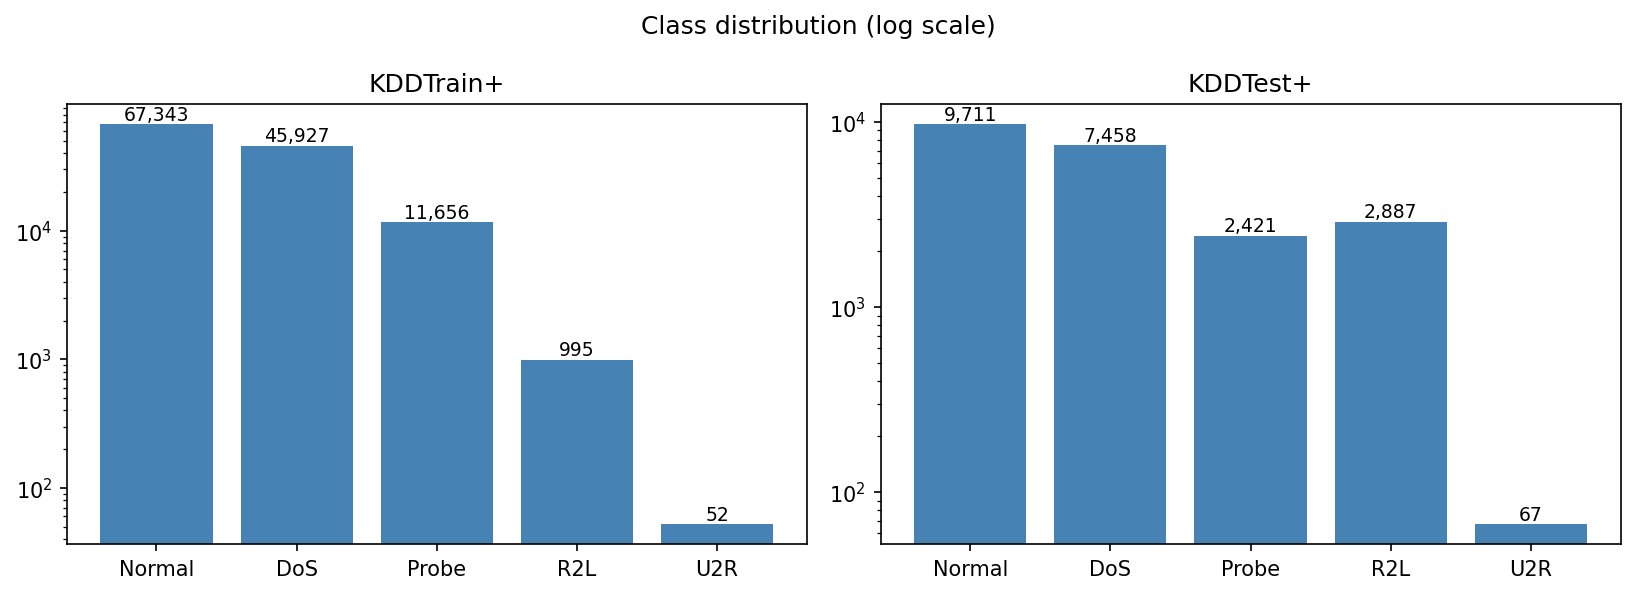
\includegraphics[width=0.9\textwidth]{class_distribution.png}
\caption{Class distribution on a log scale. There are roughly three orders of magnitude separating Normal/DoS from U2R.}
\label{fig:class-dist}
\end{figure}

Two things stand out.

\textbf{The training set is severely imbalanced.} Normal and DoS together account for roughly 90\% of the rows. U2R has only 52 training samples --- 0.04\% of the data. A model that simply predicts ``Normal'' for every connection would already score 53\% accuracy; this is why accuracy alone is a misleading metric on this problem.

\textbf{The test set has more rare attacks than the training set} relative to its size. R2L is 0.79\% of training but 12.81\% of testing. This is not a mistake. NSL-KDD's test set deliberately includes attack subtypes that are absent or under-represented in training, so that test performance reflects how the model handles \emph{novel} attacks rather than just memorised ones. This design is what makes NSL-KDD harder than its predecessor and is responsible for the cross-validation-vs-test-score gap discussed in Section~\ref{sec:results}.

\subsection{Attack Categories Explained}
\begin{itemize}
    \item \textbf{Denial of Service (DoS).} The attacker floods a service with so much traffic that legitimate users can't reach it. Examples in NSL-KDD: \texttt{neptune} (SYN flood), \texttt{smurf}, \texttt{teardrop}.
    \item \textbf{Probe.} Reconnaissance --- the attacker scans the network looking for weak spots. Examples: \texttt{nmap}, \texttt{portsweep}, \texttt{satan}.
    \item \textbf{Remote-to-Local (R2L).} The attacker is on an external machine and tries to gain access to an internal one, e.g.\ via password guessing or exploits. Examples: \texttt{guess\_passwd}, \texttt{ftp\_write}, \texttt{warezclient}.
    \item \textbf{User-to-Root (U2R).} The attacker already has a normal user account and tries to escalate to root. Examples: \texttt{buffer\_overflow}, \texttt{rootkit}, \texttt{loadmodule}.
\end{itemize}

R2L and U2R are both rare in the dataset and the most dangerous in practice, because they imply that the attacker has either gotten in (R2L) or taken control (U2R). They are also the hardest to detect from connection-level features, as the experiments will show.

%% ============================================================
\section{Methodology}
\label{sec:methodology}
%% ============================================================

\subsection{High-Level Pipeline}
The pipeline has the following stages:

\begin{center}
\texttt{Load $\to$ Encode \& Scale $\to$ Split-aware SMOTE $\to$ Train $\to$ Evaluate $\to$ Save}
\end{center}

Each stage lives in its own Python module so that swapping out a single piece (a different algorithm, a different dataset) does not break the rest. Section~\ref{sec:implementation} walks through the code; this section describes \emph{why} each step is the way it is.

\subsection{Preprocessing}
\subsubsection{Encoding categorical features}
The three categorical columns must be converted to numbers before any classifier can use them. We use one-hot encoding, which creates one new binary column per category. After encoding the dimensionality grows from 41 to 122, with most of the growth coming from the \texttt{service} column (about 70 distinct values like \texttt{http}, \texttt{ftp\_data}, \texttt{telnet}, $\dots$).

A subtle point: we encode train and test \emph{together} so that any service strings that appear only in the test set still have a column. If we encoded each split independently, the test set would have different columns from the training set and the model could not be applied.

\subsubsection{Standardisation}
After encoding, all numerical features are standardised to zero mean and unit variance, using a scaler fit \emph{only} on the training data. Standardisation matters most for Logistic Regression, which interprets coefficient sizes directly; tree-based methods do not require it but are not harmed by it. Fitting the scaler on training data only is a basic discipline rule to avoid leaking test-set distribution information into the model.

\subsection{Class Imbalance: SMOTE}
The Synthetic Minority Over-sampling Technique (SMOTE)~\cite{chawla2002} addresses class imbalance by generating synthetic minority-class samples. For a given minority sample, SMOTE picks one of its $k$ nearest neighbours from the same class and creates a new sample by interpolating between the two. Compared with simple random oversampling, this produces \emph{novel} synthetic samples rather than duplicates and reduces the risk of overfitting to a handful of minority points.

The non-obvious part of SMOTE is \emph{when} to apply it. We apply SMOTE \emph{inside each cross-validation fold}, on the training side only. Resampling the entire training set before splitting into CV folds would generate synthetic minority samples that are interpolations between the training and validation neighbours, leaking validation information back into the training set. The result is artificially inflated cross-validation scores. After cross-validation we apply SMOTE one more time on the full training set for the final model fit; the held-out KDDTest+ split is never touched by SMOTE.

\subsection{Algorithms}
Each algorithm is configured with deliberately conservative hyperparameters. Heavy tuning would cloud the comparison because each algorithm has different sensitivity to its hyperparameter space.

\subsubsection{Logistic Regression}
A linear classifier that models the log-odds of class membership as a weighted sum of features. We use the multinomial formulation (one set of weights per class) with the L-BFGS solver and \texttt{max\_iter=1000}.

\subsubsection{Random Forest}
An ensemble of decision trees~\cite{breiman2001} trained on bootstrap samples with random feature subsetting at each split. We use 100 trees with no maximum depth and \texttt{class\_weight=`balanced'} so the trees give extra weight to minority-class samples at each split. Random Forest is robust to noisy features, handles mixed feature types, and produces a feature importance score for free.

\subsubsection{XGBoost}
A gradient-boosting ensemble~\cite{chen2016} that fits trees sequentially, where each new tree is trained to correct the residual errors of the previous ensemble. We use 200 trees of maximum depth 6, learning rate 0.1, and the histogram-based tree construction algorithm for speed. XGBoost adds L1/L2 regularisation on the leaf weights and has native multi-class support via the \texttt{multi:softprob} objective.

\subsection{Evaluation}

\subsubsection{Cross-validation and held-out test}
We use stratified 5-fold cross-validation on the training set followed by a final evaluation on \texttt{KDDTest+}. Stratified folds preserve the original class proportions in each fold. ``5-fold'' (rather than the proposal's 10-fold) was chosen because at $n=125{,}973$ rows the variance of the CV estimate is already small at 5 folds, and 5-fold cuts the runtime roughly in half. We report mean and standard deviation across folds.

\subsubsection{Metrics}
We report the standard four metrics, both per-class and as weighted/macro averages:

\begin{align*}
\text{Precision} &= \frac{TP}{TP + FP}, \\
\text{Recall}    &= \frac{TP}{TP + FN}, \\
F_1              &= 2 \cdot \frac{\text{Precision} \cdot \text{Recall}}{\text{Precision} + \text{Recall}}, \\
\text{Accuracy}  &= \frac{TP + TN}{\text{Total}}.
\end{align*}

We additionally compute one-versus-rest ROC-AUC. The most informative single number on imbalanced data is \emph{macro F1}, which averages per-class F1 scores equally; weighted F1 weights by class support and tends to reward majority-class accuracy.

%% ============================================================
\section{Implementation}
\label{sec:implementation}
%% ============================================================

\subsection{Project Layout}
\begin{lstlisting}[language=bash, basicstyle=\ttfamily\small, numbers=none]
machine_learning/
  src/
    config.py           # Paths, label maps, hyperparameters
    data_loader.py      # Load NSL-KDD, map 22 attacks to 5 classes
    preprocess.py       # One-hot encode + scale + label encode
    models.py           # Define LR, RF, XGBoost
    evaluate.py         # Metrics, confusion matrix, plots
    run_experiments.py  # Entry point
  dataset/
    archive/nsl-kdd/    # KDDTrain+.txt, KDDTest+.txt
  results/              # Per-model JSON + comparison.csv
  figures/              # Class distribution, CMs, FI plots
  requirements.txt
  .venv/                # Virtual environment
\end{lstlisting}

The split into modules follows the principle that each file should have one job. Swapping NSL-KDD for CICIDS2017 in the future would only require changes to \texttt{data\_loader.py}; nothing else needs to know.

\subsection{Loading and Label Mapping}
The 22 specific attack labels in the raw NSL-KDD files are mapped to the 5-class taxonomy via a dictionary in \texttt{config.py}. The loader drops the difficulty score (we do not use difficulty stratification in this study) and applies the mapping.

\begin{lstlisting}[caption={Loading and 5-class mapping (data\_loader.py).}]
def _load_split(path):
    df = pd.read_csv(path, header=None, names=NSL_KDD_COLUMNS)
    df = df.drop(columns=["difficulty"])
    df["label"] = df["label"].map(
        lambda x: ATTACK_TO_CATEGORY.get(x, "R2L")
    )
    return df

def load_nsl_kdd():
    train_df = _load_split(TRAIN_FILE)
    test_df = _load_split(TEST_FILE)
    return train_df, test_df
\end{lstlisting}

\subsection{Preprocessing}
\begin{lstlisting}[caption={One-hot encoding over the union of train/test categories (preprocess.py).}]
def encode_features(train_df, test_df):
    X_train, y_train = _split_xy(train_df)
    X_test,  y_test  = _split_xy(test_df)
    combined = pd.concat([X_train, X_test], keys=["train", "test"])
    combined_encoded = pd.get_dummies(
        combined,
        columns=CATEGORICAL_FEATURES,
        drop_first=False,
    ).astype(np.float32)
    X_train_enc = combined_encoded.loc["train"].reset_index(drop=True)
    X_test_enc  = combined_encoded.loc["test"].reset_index(drop=True)
    return X_train_enc, y_train, X_test_enc, y_test
\end{lstlisting}

The reason we encode over the concatenation rather than fitting an encoder on train alone is documented in the module's docstring: rare \texttt{service} strings appear only in the test set and must still be representable.

\subsection{Per-Fold SMOTE}
The non-trivial part of the experiment loop is making sure SMOTE only resamples the training side of each CV fold.

\begin{lstlisting}[caption={Stratified k-fold CV with SMOTE inside each fold (run\_experiments.py).}]
def cv_with_smote(model, X, y, cv_folds=CV_FOLDS):
    skf = StratifiedKFold(n_splits=cv_folds, shuffle=True,
                          random_state=RANDOM_SEED)
    fold_scores = []
    for fold_idx, (tr_idx, va_idx) in enumerate(skf.split(X, y), 1):
        X_tr, X_va = X[tr_idx], X[va_idx]
        y_tr, y_va = y[tr_idx], y[va_idx]

        # SMOTE k_neighbors must be <= (smallest class count - 1).
        min_count = pd.Series(y_tr).value_counts().min()
        k = max(1, min(5, min_count - 1))
        sm = SMOTE(random_state=RANDOM_SEED, k_neighbors=k)
        X_tr_res, y_tr_res = sm.fit_resample(X_tr, y_tr)

        m = clone(model)
        m.fit(X_tr_res, y_tr_res)
        y_pred = m.predict(X_va)
        fold_scores.append(
            f1_score(y_va, y_pred, average="weighted",
                     zero_division=0)
        )
    return np.mean(fold_scores), np.std(fold_scores)
\end{lstlisting}

The defensive clamp on \texttt{k\_neighbors} matters because if a fold happens to have very few U2R samples, SMOTE's default \texttt{k=5} is too high and the algorithm crashes.

\subsection{Models}
\begin{lstlisting}[caption={Three classifiers under comparison (models.py).}]
def build_models():
    return {
        "Logistic Regression": LogisticRegression(
            max_iter=1000,
            solver="lbfgs",
            random_state=RANDOM_SEED,
        ),
        "Random Forest": RandomForestClassifier(
            n_estimators=100,
            max_depth=None,
            n_jobs=-1,
            random_state=RANDOM_SEED,
            class_weight="balanced",
        ),
        "XGBoost": XGBClassifier(
            n_estimators=200,
            max_depth=6,
            learning_rate=0.1,
            objective="multi:softprob",
            num_class=5,
            tree_method="hist",
            n_jobs=-1,
            random_state=RANDOM_SEED,
            eval_metric="mlogloss",
        ),
    }
\end{lstlisting}

\subsection{Evaluation Utilities}
The evaluation module computes overall metrics, per-class tables, and saves confusion matrices and feature importance plots to the \texttt{figures/} directory. Per-class precision, recall, and F1 are computed via \texttt{classification\_report} from scikit-learn. ROC-AUC is computed under the one-versus-rest binarisation.

\subsection{Reproducibility}
Every random source is seeded (\texttt{RANDOM\_SEED=42}). The full experiment runs with:
\begin{lstlisting}[language=bash, basicstyle=\ttfamily\small, numbers=none]
python3 -m venv .venv
.venv/bin/pip install -r requirements.txt
PYTHONPATH=src .venv/bin/python src/run_experiments.py
\end{lstlisting}

\subsection{Project Resources}
\label{sec:repo}
All code, LaTeX sources for this report and the accompanying IEEE-format research paper, generated figures, per-model result files, the runnable Jupyter notebook, and a recorded screencast of the pipeline executing are publicly accessible:

\begin{itemize}[leftmargin=2.2em]
    \item \textbf{Source code repository} (GitHub):\\
          \url{https://github.com/SudipAdh/NETWORK-INTRUSION-DETECTION}
    \item \textbf{Demo screencast} (Google Drive):\\
          \url{https://drive.google.com/file/d/12qWAM443JASkQnvJphx7Uv3OxtabJP6s/view?usp=sharing}
    \item \textbf{IEEE research paper:} \texttt{research\_paper/paper.pdf} in the repository.
    \item \textbf{Runnable Jupyter notebook:} \texttt{notebooks/NID\_pipeline.ipynb} in the repository.
\end{itemize}

The repository mirrors the layout described in this report (\texttt{src/}, \texttt{notebooks/}, \texttt{figures/}, \texttt{results/}, \texttt{assignment\_report/}, \texttt{research\_paper/}). The NSL-KDD dataset itself is not redistributed in the public repository and must be downloaded separately from Kaggle or the University of New Brunswick --- the README documents both. The submitted coursework zip, on the other hand, contains the dataset for offline marker access.

%% ============================================================
\section{Results and Discussion}
\label{sec:results}
%% ============================================================

\subsection{Overall Comparison}
Table~\ref{tab:overall} summarises the held-out test results.

\begin{table}[H]
\centering
\caption{Overall performance on KDDTest+. CV F1 is the mean weighted F1 across 5 folds on the training set.}
\label{tab:overall}
\begin{tabular}{lcccccc}
\toprule
Algorithm & Acc.\,(\%) & Wt.\,F1 & Macro\,F1 & ROC-AUC & CV F1 & Time (s) \\
\midrule
Logistic Regression & 77.91 & 0.7631 & 0.5745 & 0.8970 & 0.9756 & 330.3 \\
Random Forest       & 75.05 & 0.7112 & 0.5382 & 0.9476 & 0.9987 & 53.8 \\
XGBoost             & \textbf{78.66} & 0.7582 & \textbf{0.6337} & \textbf{0.9537} & 0.9991 & 90.1 \\
\bottomrule
\end{tabular}
\end{table}

XGBoost wins on three of the four held-out metrics (accuracy, macro F1, ROC-AUC). Random Forest is the fastest to train. Logistic Regression edges out the other two on weighted F1 by less than half a percentage point but, as the per-class breakdown will show, this is largely because the weighted average gives extra credit for getting Normal and DoS right.

\subsection{The Cross-Validation versus Held-Out Gap}
The most striking number in Table~\ref{tab:overall} is not in the comparison columns at all. The \emph{cross-validation} weighted F1 scores are 0.9756, 0.9987, and 0.9991 --- effectively perfect for the two ensemble methods. The held-out test scores are 0.7631, 0.7112, and 0.7582. That is a gap of roughly 22 percentage points.

This gap is not the usual ``the model overfit to the training data'' overfitting. The training-versus-CV gap is small. The gap is between the \emph{training distribution} (from which both train and CV folds are drawn) and the \emph{test distribution}, which contains attack subtypes that are absent or rare in training. This is by design --- it is what makes NSL-KDD a hard benchmark.

The practical lesson is that papers that report only cross-validation results on NSL-KDD are not measuring what they appear to be measuring. They are measuring how well the model fits the training distribution, not how well it would generalise to a slightly different attack mix. This study reports both numbers so the gap is visible.

\subsection{Per-Class Performance}
Table~\ref{tab:perclass} presents the per-class F1 scores on KDDTest+.

\begin{table}[H]
\centering
\caption{Per-class F1-scores on KDDTest+.}
\label{tab:perclass}
\begin{tabular}{lccccc}
\toprule
Algorithm & Normal & DoS & Probe & R2L & U2R \\
\midrule
Logistic Regression & 0.8058 & \textbf{0.9028} & 0.7344 & \textbf{0.2976} & 0.1320 \\
Random Forest       & 0.7800 & 0.8447 & 0.7614 & 0.1048 & 0.2000 \\
XGBoost             & \textbf{0.8095} & 0.8788 & \textbf{0.7848} & 0.2597 & \textbf{0.4356} \\
\bottomrule
\end{tabular}
\end{table}

A few patterns emerge.

\textbf{All models do well on Normal and DoS.} F1 ranges from 0.78 to 0.90, which means these classes are largely a solved problem for any of the three models.

\textbf{All models struggle on R2L.} The best performer on this class is actually Logistic Regression (0.2976), with XGBoost in second place (0.2597). Random Forest collapses on R2L (F1 = 0.1048). The reason LR does best here is that with class-balanced training and simple linear boundaries, LR produces relatively diffuse decisions that occasionally help on noisy minority classes. The trees, particularly the bagging ensemble, are more confident in their majority-class predictions and miss more R2L cases.

\textbf{XGBoost is the only model with usable U2R detection.} Its U2R F1 of 0.4356 is more than twice that of Random Forest (0.2000) and more than triple that of LR (0.1320). The gradient boosting mechanism --- where each new tree is trained to correct the residuals of the previous ensemble --- appears to genuinely help here, because the later trees specialise in the U2R cases that earlier trees miss.

\subsection{Confusion Matrices}
Figures~\ref{fig:cm-lr}, \ref{fig:cm-rf}, and \ref{fig:cm-xgb} show the confusion matrices for each model on KDDTest+. The right-hand pane is row-normalised so the diagonal is per-class recall.

\begin{figure}[H]
\centering
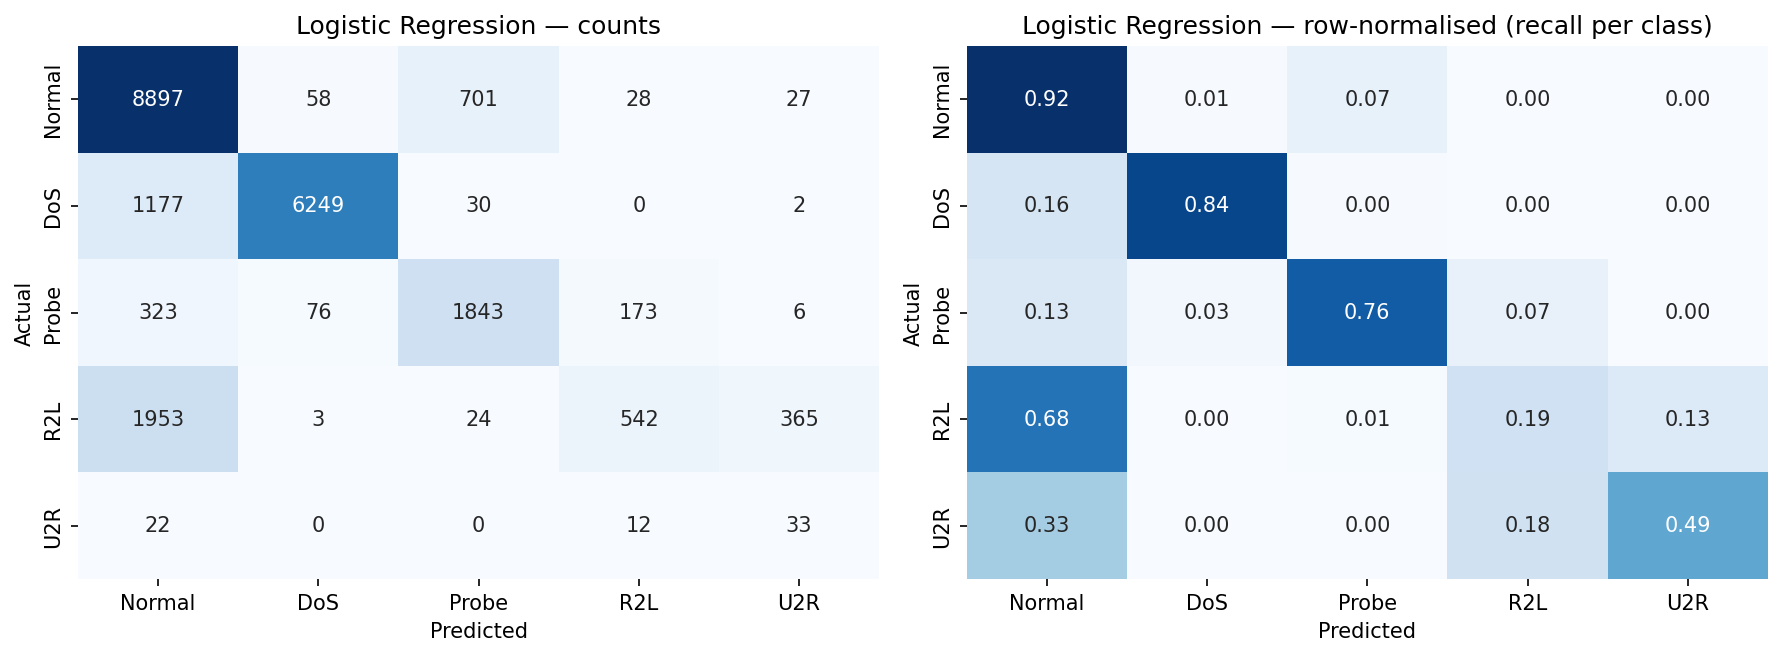
\includegraphics[width=0.95\textwidth]{cm_logistic_regression.png}
\caption{Logistic Regression confusion matrix on KDDTest+.}
\label{fig:cm-lr}
\end{figure}

\begin{figure}[H]
\centering
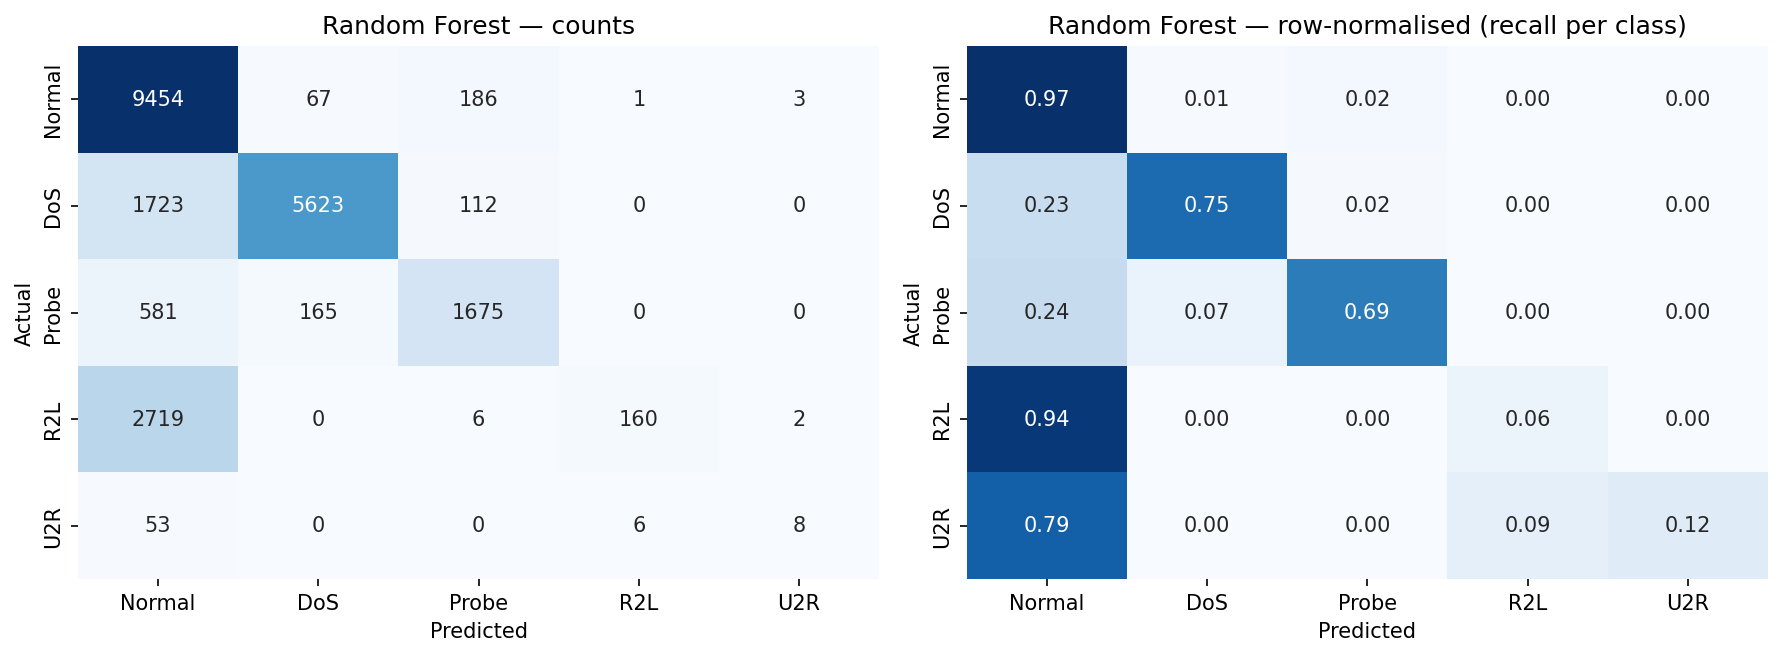
\includegraphics[width=0.95\textwidth]{cm_random_forest.png}
\caption{Random Forest confusion matrix on KDDTest+.}
\label{fig:cm-rf}
\end{figure}

\begin{figure}[H]
\centering
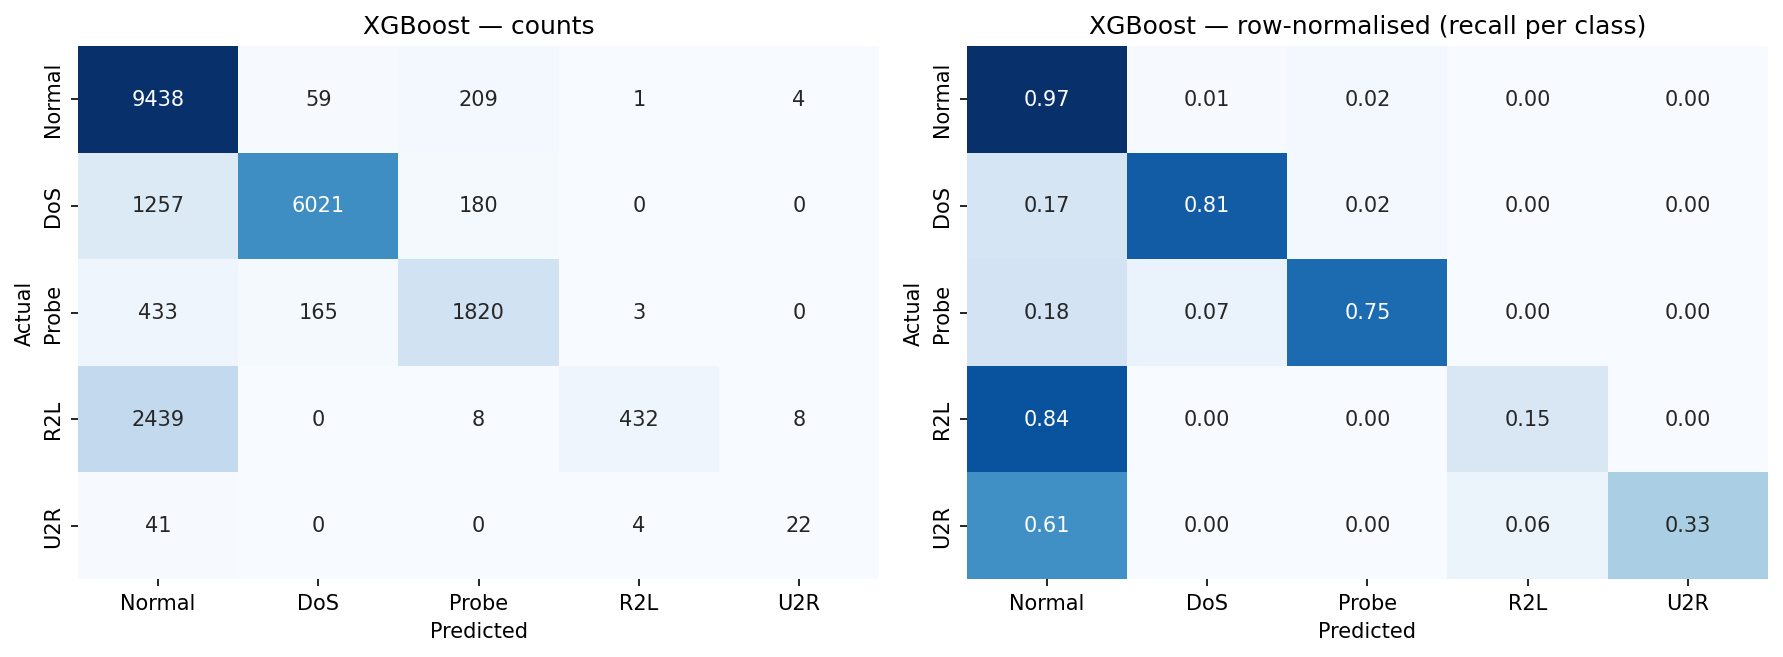
\includegraphics[width=0.95\textwidth]{cm_xgboost.png}
\caption{XGBoost confusion matrix on KDDTest+.}
\label{fig:cm-xgb}
\end{figure}

The confusion matrices give the security implication directly. Looking at the XGBoost matrix in Figure~\ref{fig:cm-xgb}, 84\% of R2L test attacks are misclassified as Normal (2{,}439 out of 2{,}887). For U2R, 61\% are misclassified as Normal (41 out of 67). These are the most dangerous attack categories in the dataset --- unauthorised remote access and privilege escalation --- and the model's most common mistake is to label them as benign traffic.

The takeaway is sobering: a deployment that relies solely on a classical-ML detector trained on NSL-KDD-style features would miss the majority of the very attacks that matter most. In production, this kind of classifier needs to be paired with anomaly detection on payloads, behavioural baselines on user accounts, or human review.

\subsection{Feature Importance}
Random Forest and XGBoost both produce feature importance scores. For Logistic Regression we use the mean absolute coefficient across classes as a rough analogue. Figure~\ref{fig:fi-xgb} shows the top 15 features as ranked by XGBoost.

\begin{figure}[H]
\centering
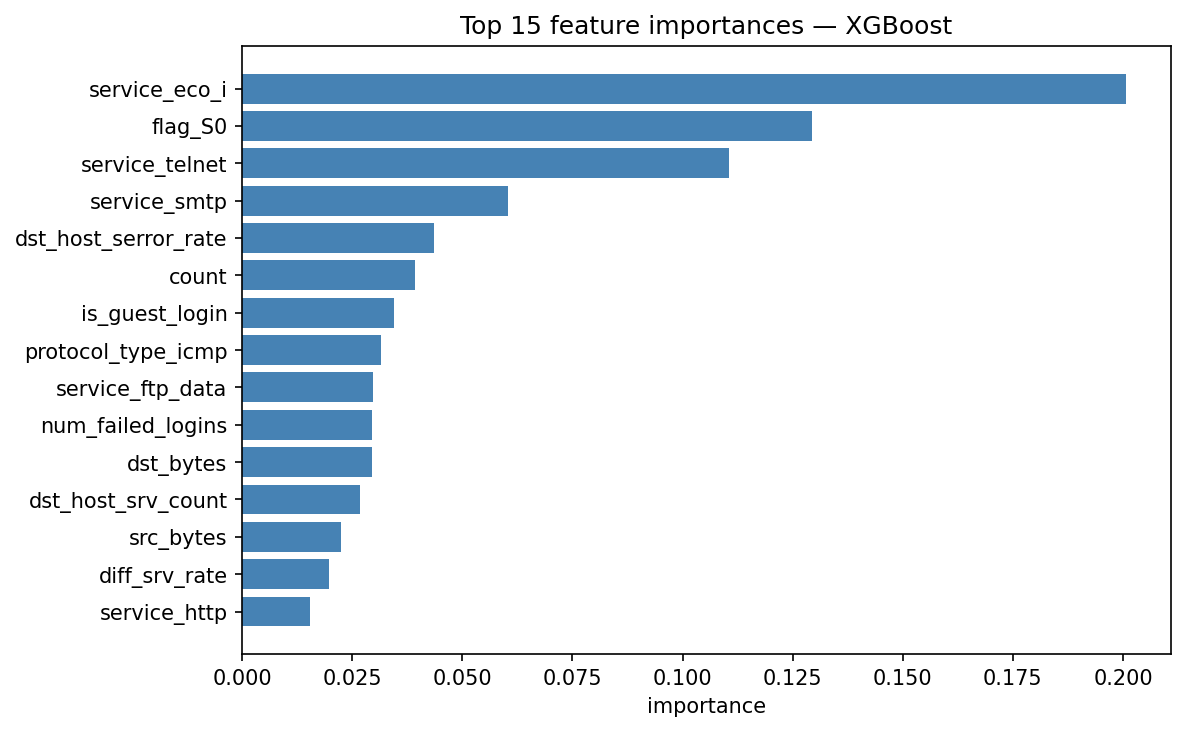
\includegraphics[width=0.85\textwidth]{fi_xgboost.png}
\caption{Top 15 feature importances from XGBoost.}
\label{fig:fi-xgb}
\end{figure}

The top features are interpretable.

\begin{itemize}
    \item \texttt{service\_eco\_i} ($\sim$20\% of total importance) marks ICMP echo traffic, which appears heavily in probe attacks.
    \item \texttt{flag\_S0} ($\sim$13\%) marks connections where a SYN was sent but no SYN-ACK returned --- the canonical signature of SYN floods and port scans.
    \item \texttt{service\_telnet} ($\sim$11\%) flags Telnet activity, which is rare in legitimate modern environments and shows up in R2L brute-force attempts.
    \item \texttt{service\_smtp} ($\sim$6\%) flags mail traffic, which figures in some R2L and DoS variants.
    \item \texttt{dst\_host\_serror\_rate} ($\sim$5\%) is the rate of connection errors to a target host --- another classic scanning signature.
\end{itemize}

The first three features alone account for roughly 40\% of the model's split decisions. This is a useful practical result: an analyst running a small monitoring deployment could focus on these few quantities and capture most of what the trained model would. The trained model adds value by quantifying their interaction with thirty-eight other signals, but the headline features are exactly what a security textbook would tell you to watch.

\subsection{Wall-Clock Time}
Random Forest is the fastest of the three (53.8 s end-to-end including 5-fold CV), XGBoost is intermediate (90.1 s), and Logistic Regression is, surprisingly, the slowest (330.3 s). The reason LR is slow is that after SMOTE the training set grows from 125{,}973 to 336{,}715 rows, and on 122 features the L-BFGS optimiser requires many passes over this larger matrix to converge to a strict tolerance. Tree-based methods, by contrast, scan each feature once per split and parallelise easily across cores. This is a useful counterintuition --- ``simple'' linear models are not always faster than ``complex'' ensembles.

\subsection{Summary of Findings}
\begin{enumerate}
    \item \textbf{XGBoost is the best overall model on this benchmark}, winning on accuracy, macro F1, ROC-AUC, and rare-class detection.
    \item \textbf{All three models are strong on Normal and DoS} (F1 $>$ 0.78) but weak on R2L (F1 $\leq$ 0.30).
    \item \textbf{The 22-percentage-point CV-vs-test gap} is the single largest effect in the experiment and matters more than the differences between models.
    \item \textbf{Macro F1 is the right headline metric} on imbalanced data; weighted F1 and accuracy hide the rare-class failures.
    \item \textbf{A few features carry most of the signal} (\texttt{service\_eco\_i}, \texttt{flag\_S0}, \texttt{service\_telnet}). This is reassuring for interpretability.
\end{enumerate}

%% ============================================================
\section{Limitations and Future Work}
\label{sec:limitations}
%% ============================================================

This study has clear limitations.

\textbf{Single dataset.} All conclusions are drawn from NSL-KDD. The underlying network traffic is from 1998 and lacks modern attack patterns: HTTP-based exploits, encrypted-channel exfiltration, modern DDoS, web shells, modern botnets. A natural follow-up is to retrain the same pipeline on CICIDS2017~\cite{panigrahi2018}, a 2017 benchmark with $\sim$2.8 million labelled flows and 14 attack categories including Heartbleed, Botnet, and Web Attacks. We have left a placeholder \texttt{data\_loader} for this work.

\textbf{Classical algorithms only.} We do not compare against deep learning. Existing literature suggests that on NSL-KDD, well-tuned classical models are competitive with deep models in accuracy while being orders of magnitude faster to train. On larger, modern benchmarks like CICIDS2017 the picture changes; deep learning would be a sensible next step.

\textbf{Conservative hyperparameters.} We did not run a hyperparameter search. The trade-off is that aggressive tuning of one model would distort the comparison. With more compute, a Bayesian or grid search per model with the same budget for each would tighten the numbers but probably not change the qualitative ranking.

\textbf{Single resampling strategy.} We only used SMOTE. ADASYN, Borderline-SMOTE, SMOTE-Tomek, and undersampling techniques would each give slightly different rare-class behaviour. Cost-sensitive learning --- adjusting the loss so that rare-class errors are penalised more --- is a particularly interesting direction we did not explore.

\textbf{R2L detection remains poor.} The strongest model in the study still recalls only 15\% of R2L attacks on the test set. This is a fundamental limit of connection-level features for R2L-style attacks, where the malicious behaviour lives in the payload (e.g.\ password attempts, exploit strings) rather than in connection statistics. A production system would augment this kind of model with payload inspection or behavioural baselining.

%% ============================================================
\section{Social, Ethical, Legal, and Professional Considerations}
\label{sec:ethics}
%% ============================================================

A network intrusion detector is not a neutral piece of software, and any honest report on building one should make its non-technical implications explicit.

\subsection{Privacy}
Even when an IDS examines only flow-level metadata --- packet counts, protocol flags, byte volumes, connection durations --- the activity is still a form of surveillance. The features used in this study are metadata only, not packet payloads, but a deployed IDS can still profile user behaviour in fine detail. A responsible deployment must minimise data retention, segregate IDS logs from identifiable user data wherever possible, and disclose monitoring practice to users in privacy notices.

\subsection{False Positives and Asymmetric Harm}
The errors made by an ML detector are not symmetric in their human impact. A false negative may let an attack through; a false positive can lock a legitimate user out of a service or escalate to a human investigation that is itself intrusive. The 60--80\% false-negative rate observed for R2L and U2R in this study (Section~\ref{sec:results}) means classical-ML IDS should never be the sole defence against these attack families; layered detection (host-based, behavioural, payload-inspection) is required to compensate. Equally, an over-tuned model that flags too many connections becomes operational noise that analysts will eventually ignore --- sometimes called ``alert fatigue'' --- and a noisy detector can be more dangerous than no detector at all.

\subsection{Bias and Dataset Provenance}
NSL-KDD's underlying traffic comes from the DARPA 1998 simulation, which represents US-military network conditions of nearly three decades ago. A detector trained on this data inherits its blind spots: encrypted traffic is absent, modern application-layer attacks (HTTP-based exploits, modern phishing infrastructure) are not represented, and the geographic and linguistic diversity of more recent traffic is missing. A Nepal-deployed system trained on NSL-KDD alone would be likely to under-detect locally relevant attack patterns. A responsible production deployment would require fine-tuning on representative local traffic, not direct transplantation.

\subsection{Legal Context}
In Nepal, network monitoring is governed by the \emph{Electronic Transactions Act 2008} and the \emph{Privacy Act 2018}, both of which require lawful basis and proportionality for processing communications data. International deployments would additionally need to consider GDPR Article~6 (lawful basis) and Article~32 (security of processing). The use of synthetic data (SMOTE) for training does not by itself raise additional legal exposure --- synthetic samples do not contain real user information --- but the underlying training data does, so retention and access controls apply to it. Cross-border transfer of training data raises additional questions that must be cleared before deployment.

\subsection{Professional Responsibility}
Reporting only cross-validation scores --- the convenient but misleading number that many NSL-KDD papers quote --- misrepresents what a model can do once deployed. Professional integrity requires that practitioners separate distribution-fitting performance from generalisation performance and communicate the difference to non-technical decision makers. This report takes that requirement seriously, which is why both numbers are reported and why the gap between them is discussed at length. More broadly, deploying an IDS without complementary controls (logging governance, incident response plans, transparent appeal mechanisms for users flagged by the system) is professionally negligent regardless of how accurate the model itself is.

%% ============================================================
\section{Conclusion}
\label{sec:conclusion}
%% ============================================================

This project compared three classical machine learning algorithms --- Logistic Regression, Random Forest, and XGBoost --- on the full five-class NSL-KDD intrusion detection problem under identical preprocessing and evaluation conditions. The pipeline was reproducible end-to-end: 5-fold cross-validation with SMOTE applied per fold, a held-out evaluation on the official test split, and per-class metrics throughout. XGBoost emerged as the strongest model on the held-out test set (78.66\% accuracy, 0.6337 macro F1, 0.9537 ROC-AUC) and was the only model with credible U2R detection (F1 = 0.4356). Logistic Regression was unexpectedly strong on R2L by virtue of class-balanced training; Random Forest was fastest to train but weakest on rare classes.

Two findings deserve more emphasis than they are usually given in NSL-KDD studies. The first is the 22-percentage-point gap between cross-validation and held-out test scores --- a property of NSL-KDD's deliberate inclusion of unseen attack subtypes in the test set, and a number that papers reporting only CV results are quietly hiding. The second is that all three models, even the best, miss the large majority of R2L attacks. Classical-ML detectors trained on connection-level features should not be deployed as the sole line of defence against R2L-style threats.

What I learned from doing the project is more practical than the numbers themselves. The amount of work that goes into a fair comparison --- making sure preprocessing is identical across models, that SMOTE is applied per fold rather than once at the start, that the test set is never touched until the very end --- is much greater than the work of running each algorithm in isolation. Many of the published NSL-KDD studies skip one or more of these steps and still report ``state-of-the-art'' numbers; once you do the careful version, the numbers are lower but defensible. For the same effort that produces a single mediocre paper, a careful pipeline produces something that can be extended to other datasets, other algorithms, and other evaluation settings without rewriting from scratch.

%% ============================================================
\section*{References}
\addcontentsline{toc}{section}{References}
%% ============================================================

\begin{thebibliography}{99}

\bibitem{tavallaee2009}
M. Tavallaee, E. Bagheri, W. Lu, and A. A. Ghorbani, ``A detailed analysis of the KDD CUP 99 data set,'' \emph{Proc. IEEE Symposium on Computational Intelligence for Security and Defense Applications (CISDA)}, pp. 1--6, 2009.

\bibitem{kdd99}
KDD Cup 1999 Data, UCI Machine Learning Repository. \url{http://kdd.ics.uci.edu/databases/kddcup99/kddcup99.html}

\bibitem{chawla2002}
N. V. Chawla, K. W. Bowyer, L. O. Hall, and W. P. Kegelmeyer, ``SMOTE: Synthetic Minority Over-sampling Technique,'' \emph{Journal of Artificial Intelligence Research}, vol. 16, pp. 321--357, 2002.

\bibitem{breiman2001}
L. Breiman, ``Random forests,'' \emph{Machine Learning}, vol. 45, no. 1, pp. 5--32, 2001.

\bibitem{chen2016}
T. Chen and C. Guestrin, ``XGBoost: A scalable tree boosting system,'' \emph{Proc. 22nd ACM SIGKDD International Conference on Knowledge Discovery and Data Mining}, pp. 785--794, 2016.

\bibitem{ahmad2021}
Z. Ahmad, A. S. Khan, C. W. Shiang, J. Abdullah, and F. Ahmad, ``Network intrusion detection system: A systematic study of machine learning and deep learning approaches,'' \emph{Transactions on Emerging Telecommunications Technologies}, vol. 32, no. 1, e4150, 2021.

\bibitem{dhanabal2015}
L. Dhanabal and S. P. Shantharajah, ``A study on NSL-KDD dataset for intrusion detection system based on classification algorithms,'' \emph{International Journal of Advanced Research in Computer and Communication Engineering}, vol. 4, no. 6, pp. 446--452, 2015.

\bibitem{ingre2015}
B. Ingre and A. Yadav, ``Performance analysis of NSL-KDD dataset using ANN,'' \emph{Proc. International Conference on Signal Processing and Communication Engineering Systems (SPACES)}, pp. 92--96, 2015.

\bibitem{gu2021}
J. Gu and S. Lu, ``An effective intrusion detection approach using SVM with na\"ive Bayes feature embedding,'' \emph{Computers \& Security}, vol. 103, p. 102158, 2021.

\bibitem{panigrahi2018}
R. Panigrahi and S. Borah, ``A detailed analysis of CICIDS2017 dataset for designing intrusion detection systems,'' \emph{International Journal of Engineering \& Technology}, vol. 7, no. 3.24, pp. 479--482, 2018.

\bibitem{nature2026}
``Anomaly-based intrusion detection on benchmark datasets for network security: a comprehensive evaluation,'' \emph{Scientific Reports}, vol. 16, 2026.

\bibitem{applied2025}
``Advanced IDS: a comparative study of datasets and machine learning algorithms for network flow-based intrusion detection systems,'' \emph{Applied Intelligence}, 2025.

\bibitem{sklearn}
F. Pedregosa et al., ``Scikit-learn: Machine Learning in Python,'' \emph{Journal of Machine Learning Research}, vol. 12, pp. 2825--2830, 2011.

\end{thebibliography}

%% ============================================================
\appendix
\section*{Appendix A: Environment and Reproduction}
\addcontentsline{toc}{section}{Appendix A: Environment and Reproduction}
%% ============================================================

\textbf{Python:} 3.13.2

\textbf{Required libraries (\texttt{requirements.txt}):}
\begin{lstlisting}[language=bash, basicstyle=\ttfamily\small, numbers=none]
pandas
numpy
scikit-learn
matplotlib
seaborn
xgboost
imbalanced-learn
joblib
\end{lstlisting}

\textbf{macOS dependency:} XGBoost requires OpenMP. Install with \texttt{brew install libomp}.

\textbf{Reproducing the experiment:}
\begin{lstlisting}[language=bash, basicstyle=\ttfamily\small, numbers=none]
# 1. Create the virtual environment
python3 -m venv .venv
.venv/bin/pip install -r requirements.txt

# 2. Run the full pipeline
PYTHONPATH=src .venv/bin/python src/run_experiments.py
\end{lstlisting}

The script writes to \texttt{results/} (one JSON and one CSV per model, plus the master \texttt{comparison.csv}) and to \texttt{figures/} (class distribution, three confusion matrices, three feature importance plots). All randomness is seeded with \texttt{RANDOM\_SEED=42}.

\textbf{Source code:} The complete project --- code, reports, figures, and per-model results --- is hosted at \url{https://github.com/SudipAdh/NETWORK-INTRUSION-DETECTION}. Clone the repository, place the NSL-KDD train/test files under \texttt{dataset/archive/} (download links in the README), and run the command above to reproduce every figure and table in this report.

\section*{Appendix B: Selected Code Listings}
\addcontentsline{toc}{section}{Appendix B: Selected Code Listings}

\subsection*{B.1: Configuration (\texttt{config.py})}
\begin{lstlisting}[caption={Central configuration: paths, label maps, hyperparameters.}]
RANDOM_SEED = 42
CV_FOLDS = 5
CATEGORICAL_FEATURES = ["protocol_type", "service", "flag"]
CLASS_LABELS = ["Normal", "DoS", "Probe", "R2L", "U2R"]
ATTACK_TO_CATEGORY = {
    "normal": "Normal",
    "back": "DoS", "neptune": "DoS", "smurf": "DoS", ...,
    "ipsweep": "Probe", "nmap": "Probe", "satan": "Probe", ...,
    "ftp_write": "R2L", "guess_passwd": "R2L", ...,
    "buffer_overflow": "U2R", "rootkit": "U2R", ...,
}
\end{lstlisting}

\subsection*{B.2: End-to-End Driver (\texttt{run\_experiments.py})}
\begin{lstlisting}[caption={Main pipeline: load -> preprocess -> CV+SMOTE -> final fit -> test eval.}]
def main():
    train_df, test_df = load_nsl_kdd()
    plot_class_distribution(train_df, test_df, ...)

    X_train, y_train, X_test, y_test, feature_names, _ = (
        full_pipeline(train_df, test_df)
    )

    sm = SMOTE(random_state=RANDOM_SEED, k_neighbors=5)
    X_train_smote, y_train_smote = sm.fit_resample(X_train, y_train)

    for name, model in build_models().items():
        cv_mean, cv_std = cv_with_smote(model, X_train, y_train)
        model.fit(X_train_smote, y_train_smote)
        y_pred  = model.predict(X_test)
        y_proba = model.predict_proba(X_test)
        overall = overall_metrics(y_test, y_pred, y_proba)
        per_class = per_class_table(y_test, y_pred)
        save_results(name, overall, per_class, predictions=y_pred)
        plot_confusion_matrix(y_test, y_pred, name, ...)
        plot_feature_importance(feature_names, ..., name, ...)
\end{lstlisting}

\section*{Appendix C: Full Per-Class Tables}
\addcontentsline{toc}{section}{Appendix C: Full Per-Class Tables}

\begin{table}[H]
\centering
\caption{Logistic Regression --- per-class results on KDDTest+.}
\begin{tabular}{lcccr}
\toprule
        & precision & recall & f1-score & support \\
\midrule
Normal  & 0.7191 & 0.9162 & 0.8058 & 9{,}711 \\
DoS     & 0.9785 & 0.8379 & 0.9028 & 7{,}458 \\
Probe   & 0.7094 & 0.7613 & 0.7344 & 2{,}421 \\
R2L     & 0.7179 & 0.1877 & 0.2976 & 2{,}887 \\
U2R     & 0.0762 & 0.4925 & 0.1320 &      67 \\
\bottomrule
\end{tabular}
\end{table}

\begin{table}[H]
\centering
\caption{Random Forest --- per-class results on KDDTest+.}
\begin{tabular}{lcccr}
\toprule
        & precision & recall & f1-score & support \\
\midrule
Normal  & 0.6507 & 0.9735 & 0.7800 & 9{,}711 \\
DoS     & 0.9604 & 0.7540 & 0.8447 & 7{,}458 \\
Probe   & 0.8464 & 0.6919 & 0.7614 & 2{,}421 \\
R2L     & 0.9581 & 0.0554 & 0.1048 & 2{,}887 \\
U2R     & 0.6154 & 0.1194 & 0.2000 &      67 \\
\bottomrule
\end{tabular}
\end{table}

\begin{table}[H]
\centering
\caption{XGBoost --- per-class results on KDDTest+.}
\begin{tabular}{lcccr}
\toprule
        & precision & recall & f1-score & support \\
\midrule
Normal  & 0.6936 & 0.9719 & 0.8095 & 9{,}711 \\
DoS     & 0.9641 & 0.8073 & 0.8788 & 7{,}458 \\
Probe   & 0.8209 & 0.7518 & 0.7848 & 2{,}421 \\
R2L     & 0.9818 & 0.1496 & 0.2597 & 2{,}887 \\
U2R     & 0.6471 & 0.3284 & 0.4356 &      67 \\
\bottomrule
\end{tabular}
\end{table}

%% ============================================================
\section*{Appendix D: Per-Fold Cross-Validation Evidence}
\addcontentsline{toc}{section}{Appendix D: Per-Fold Cross-Validation Evidence}
%% ============================================================

Table~\ref{tab:cvfolds} reports the weighted F1 score on each fold of the 5-fold stratified cross-validation, after per-fold SMOTE resampling, for each of the three algorithms. The very small standard deviation (between 0.0002 and 0.0015) indicates that fold-to-fold variation is negligible compared to the gap with held-out test performance --- which reinforces the claim in Section~\ref{sec:results} that the CV-vs-test gap is a property of the dataset, not statistical noise.

\begin{table}[H]
\centering
\caption{Per-fold weighted F1 on the NSL-KDD training set (5-fold stratified CV with SMOTE applied per fold).}
\label{tab:cvfolds}
\begin{tabular}{lccccc|cc}
\toprule
Algorithm & Fold 1 & Fold 2 & Fold 3 & Fold 4 & Fold 5 & Mean & Std \\
\midrule
Logistic Regression & 0.9777 & 0.9766 & 0.9750 & 0.9735 & 0.9753 & 0.9756 & 0.0015 \\
Random Forest       & 0.9988 & 0.9987 & 0.9989 & 0.9987 & 0.9984 & 0.9987 & 0.0002 \\
XGBoost             & 0.9990 & 0.9991 & 0.9994 & 0.9991 & 0.9988 & 0.9991 & 0.0002 \\
\bottomrule
\end{tabular}
\end{table}

These numbers were captured directly from the experiment log file (\texttt{results/run.log}), which is also published in the GitHub repository.

\end{document}
